\section{Daniel Falk}
\subsection{Inledning}
Jag har i detta projekt haft rollen som analysansvarig vilket innebär en analys av kundens behov och framställning av krav utifrån dessa. Rapporten beskriver hur kravframställningen gått till i detta projekt och hur prototyper har använts för att kommunicera idéer.
\subsubsection{Syfte}
Syftet med denna del av rapporten är att ta reda på hur man kan samla in krav som kunden har på produkten. Fokus ligger på användningen av prototyper med utgångspunkt i detta projekt.
\subsubsection{Frågeställning}
Hur kan man samla in krav som tillfredställer kundens verkliga behov?
Hur kan man arbeta med prototyper för att framställa krav?
\subsubsection{Avgränsningar}
Rapporten har sin utgångspunkt i hur kravframställningen gått till i detta projekt. Metoden bör inte ses som ett allmänt tillvägagångssätt.
\subsection{Bakgrund}
Att förstå kundens verkliga behov utgör grunden för ett lyckat projekt. Ett projekt faller ofta på grund av dålig kravframställning. %(någon referens). 
\subsection{Teori}
Teorin beskriver kravinsamlingsmetoder, verktyg och vilka problem som kan uppstå vid kravframställning. 
\subsubsection{Problem}
Det finns ett antal barriärer som kan uppstå vid kravframställning. Ett problem är ofta att kunden inte kan formulera vad de vill ha. De kan se problemet men inte vad som behöver göras. De kan överdriva vissa problem medan andra förbises. 
Ett annat problem är att kunden kan ha fastnat i ett invant mönster. De kan ha svårt att föreställa sig nya sätt att utföra en uppgift på.
\cite{Lauesen} %%Kolla upp om denna parafras är ok.

\subsubsection{Vertktyg}
Prototyper
\subsubsection{Kravinsamlingsmetoder}
\subsection{Metod}
Denna del beskriver hur kravframställningen gått till i detta projekt. Först beskrivs arbetet med att analysera kundens behov under förstudien. Vidare beskrivs mer ingående vilka metoder som använts och hur kraven valdes att representeras. Avslutningsvis beskrivs vilka användartester som genomfördes och hur dessa bedrog till utvecklingen.
\subsubsection{Förstudie}
Den största delen utav analysarbetet skedde under förstudien. Här identifierades de olika intressenterna och en kravspecifikation utarbetades. Våran första kontakt med projektet var en projektbeskrivning där kunden formulerade sina mål och visioner av projektet. Några vikta krav gavs också såsom att prototypdesign skulle genomföras i samarbete med kunden. Ett första möte utav fyra under förstudien gav sedan mer information och vi började våran kravinsamling. Vi kunde konstatera att vi hade två olika intressenter att arbeta med. Dels sjuksköterskorna som är användare av systemet och dels CMIT, Centrum för medicinsk teknik och IT, som ansvarar för sjukhusets IT-miljöer. För att förstå användarnas behov hölls ett studiebesök där vi fick en visning av nuvarande system och hur det används. Detta var nödvändigt för att verkligen förstå vad det var som behövde göras och vad som kunde förbättras. Från CMIT:s sida hölls mer tekniska möten där teknikval diskuterades. Här var det viktigt att ta reda på vilka begränsningar som fanns och vilka val som passade våra och deras erfarenheter.
\subsubsection{Kravinsamlingsmetoder}
För att samla in krav under möten med kund har vi dels fört anteckningar på papper eller dator och dels spelat in på mobil. När vi varit flera personer på möten har vi gått igenom och diskuterat våra anteckningar i efterhand. Vid oklarheter har vi antecknat dessa för att förtydliga med kund. Inspelning användes främst vid första mötet och var användbart då vi fick mycket information att sätta oss in i.
Kravspecifikationen skrev i Google docs. Detta valdes eftersom kraven utarbetades tillsammans med kund. Ett gemensamt redigerbart dokument gav en möjlighet för oss att arbeta på olika platser under kravframställningen vilket var effektivt. En kommentarsfunktion gav oss möjligheten att kommentera krav och föreslå förbättringar. Under interna möten och kundmöten var den gemensamma redigeringen också till nytta då kravformuleringar snabbt kunde genomföras.
\subsubsection{Kravrepresentation}
Kraven gavs en prioritetsordning för att kunna urskilja de mest väsentliga kraven. Detta kändes nödvändigt då vi var begränsade av en tidsbudget. En prioritering av kraven gav utrymme för vidareutveckling i mån av tid. Krav med prioritet 1 var att betrakta som grundkrav som skulle genomföras för att projektet skulle ses som godkänt. Krav med prioritet 2 var att betrakta som önskvärda och som skulle genomföras om då grundkraven var genomförda. Krav med prioritet 3 var krav som fångats upp med som skulle ses som framtida utbyggnad. 
%Koppla till nån litteratur/standard.

%Strukturering av krav
Kraven numrerades för att lätt kunna refereras till under projektets gång. De delades också in i olika sektioner efter deras del i systemet. Sektionerna var plocklistor, handböcker, kartotek, lagersystem. En extra sektion för generella krav användes. Denna uppdelning kändes naturlig för detta projekt. 
%Man skulle också kunna dela in dem efter blablabla...

Kravspecifikationen skrevs med stöd från standarden IEEE 830. Enligt standarden ska ett krav vara korrekt, otvetydigt, färdigt, konsekvent, prioriterat, verifierbart, modifierbart och spårbart. Detta eftersträvades men det kan diskuteras om alla krav passerar dessa filter. I slutändan var det ändå våran gemensamma förståelse för kravet tillsammans med kunden som accepterades. 

Enligt standarden uttrycktes kraven på ska-form. Ett exempel på ett krav från projektet är följande: "Plocklistor ska innehålla information om artikelns namn, förråd, sektion, hylla och fack".
\subsubsection{Prototyning}
Under förstudien valde vi att göra LoFi-prototyper som vi tog med till kund. Vid dessa tester kunde vi se om vi var på rätt bana när det gällde design och struktur. LoFi-protptyperna utjordes av enkla pappersskisser. Ett exempel visas i figur~\ref{fig:lofiprototyper}.

\begin{figure}[htbp]
\begin{center}
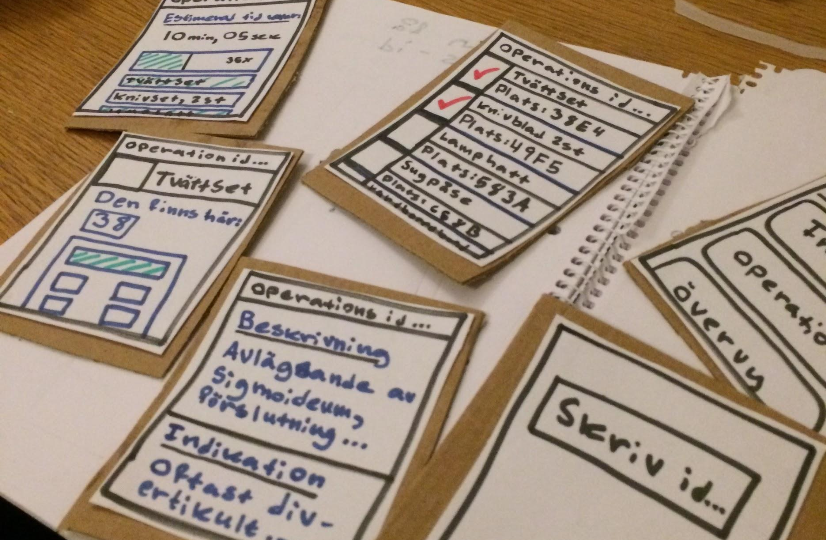
\includegraphics[scale=0.2]{lofiprototyper.png}
\caption{LoFi-prototyper}
\label{fig:lofiprototyper}
\end{center}
\end{figure}
Vi hade vid vissa tillfällen olika förslag på design och samlade då in positiva och negativa kommentaren om de olika prototyperna.



\subsubsection{Användartest}
Vid varje iterationsslut hölls ett möte med kund där vi demonstrerade nya features och lät kunden testa systemet. Iterationerna gjorde att vi snabbt kunde rätta till eventuella missförstånd. Vid dessa möten diskuterade vi också vad som skulle genomföras nästa iteration. Vi gick igenom vilka krav som var genomförda och vilka som skulle prioriteras till nästa iteration.

\subsection{Resultat}
\subsection{Diskussion}
\subsubsection{Resultat}
\subsubsection{Metod}
\subsection{Slutsatser}
\subsection{Referenser}
\vspace{-9mm}
\begin{thebibliography}{9}
\bibitem{Lauesen}
Lauesen, S. (2002) Software Requirements: Styles and Techniques. Harlow: AddisonWessly.
\end{thebibliography}

%Lauesen, S. (2002) Software Requirements: Styles and Techniques. Harlow: AddisonWessly. %Note to self:Dubbelkolla

